\documentclass{article}
\usepackage[utf8]{inputenc}
\usepackage[brazil]{babel}
\usepackage{graphicx}
\usepackage{mathtools}
\usepackage[colorlinks, linkcolor=blue, urlcolor=blue, citecolor=blue]{hyperref}
\usepackage[a4paper, left=20mm, right=20mm, top=20mm, bottom=20mm]{geometry}

\title{\textbf{DES: Data Encryption Standard \\
        \large INE5429 - Segurança em Computação}}
\author{
    Caique Rodrigues Marques \\
    {\texttt{c.r.marques@grad.ufsc.br}}
}
\date{}

\begin{document}

\maketitle

\footnotetext[1]{Para ser classificado como um
\href{https://en.wikipedia.org/wiki/Abelian\_group\#Definition}{grupo abeliano}
é necessário satisfazer cinco axiomas.}

\textbf{Nota}: As imagens usadas foram retiradas do
livro-texto\cite{stallings2014}.

\begin{enumerate}
    \item[3.2] Devido ao algoritmo de \textit{key scheduler} apenas copiar os
        primeiros 8 \textit{rounds} nos \textit{rounds} de 9 a 16, na ordem
        inversa, é possível notar que o ciframento e o deciframento do cifrador
        de Feistel são iguais. Assim, para conseguir a mensagem $m$ basta que o
        oráculo cifre $c$, assim o texto cifrado retornado vai ser o texto $c$
        decifrado, logo, a mensagem $m$.

    \item[3.7] A estrutura do DES constitui do uso da função de Feistel que é
        inversível, a partir disto é possível mostrar que o decifrador DES é o
        inverso do cifrador DES. Definindo uma função de Feistel $F$ e a
        entrada composta por ($L_{1}$, $R_{1}$), o primeiro \textit{round} do
        cifrador é definido como:
    \begin{align*}
        & L_{2} = R_{1} \oplus F(L_{1}) \\
        & R_{2} = L{1},
    \end{align*}
    onde $L_{2}$ e $R_{2}$ compõem a saída cifrada resultante. Supondo que o
        cifrador possua apenas um \textit{round}, é possível conseguir a
        entrada original apenas com a função $F$ e a saída cifrada:
    \begin{align*}
        & L_{1} = R_{2} \\
        & R_{1} = L_{2} \oplus F(L_{1}).
    \end{align*}
    Isso é possível devido a dois pontos:
    \begin{enumerate}
        \item Parte da entrada é carregada ao fim de cada \textit{round};
        \item A operação de $\oplus$ entre quaisquer dois elementos garante a
            inversibilidade, assim, 
        \begin{itemize}
            \item $A \oplus B = C$;
            \item $A \oplus C = B$;
            \item $B \oplus C = A$.
        \end{itemize}
        Tais propriedades são válidas porque o conjunto $D$, munido da operação
            de $\oplus$ entre dois elementos $a$ e $b$ quaisquer pertencentes a
            $D$, é um grupo abeliano.\footnotemark[1]
    \end{enumerate}
    Portanto, a função de Feistel F é inversível.
    
    Resta apenas as funções $IP$ e $IP^{-1}$. Ambas as funções são de
        permutações, logo, apenas rearranja os bits e, por definição, $IP^{-1}$
        é o inverso de $IP$. Para ciframento:
    \begin{itemize}
        \item O texto original é entrada da função $IP$, resultando na saída
            composta por $(L, R)$;
        \item A saída do item anterior é entrada da função de Feistel,
            resultando em $(X, Y)$;
        \item Por fim, a saída do item anterior é entrada para a função
            $IP^{-1}$, resultando no texto cifrado $c$.
    \end{itemize}
    Para deciframento:
    \begin{itemize}
        \item O texto cifrado $c$ é entrada da função $IP$, resultando na saída
            composta por $(X, Y)$;
        \item A saída do item anterior é entrada da função de Feistel,
            resultando em $(L, R)$;
        \item Por fim, a saída do item anterior é entrada para a função
            $IP^{-1}$, resultando no texto original.
    \end{itemize}
    Portanto, o deciframento DES é o inverso do ciframento DES.
    
    \item[3.12] Dadas as duas tabelas abaixo,
    \begin{figure}[ht!]
        \centering
        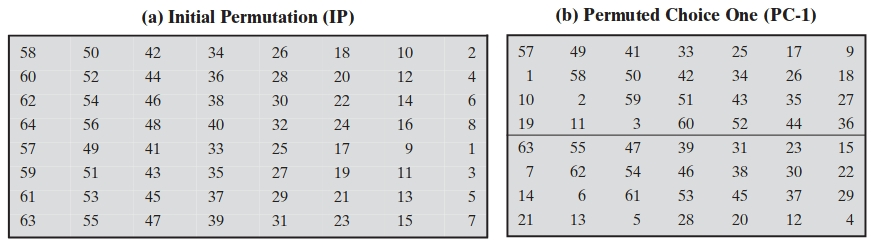
\includegraphics[width=0.8\textwidth]{imgs/tables.jpg}
        \label{fig:tables}
    \end{figure}
    a única coisa notável é que as tabelas são bem parecidas, a exceção está na
    \textit{Permuted Choice One} que possui um bit a menos que a tabela de
    \textit{Initial Permution} - ainda é possível notar alguns padrões de
    posicionamento entre ambas (começando pelo 57 em ambas, por exemplo), o que
    pode permitir alguma implementação similar da tabela \textit{IP} na
    \textit{PC-1}. De resto, não há mais nada de especial.
    
    \item[3.13] Durante o deciframento, \textit{rounds} com um 1 bit
        rotacionados são 2, 9 e 16, enquanto o restante (exceto o
        \textit{round} 1) são rotacionados 2 bits. \\
    \begin{tabular}{|l|*{16}{c}|c}
        \hline
        Número do \textit{round} & 1 & 2 & 3 & 4 & 5 & 6 & 7 & 8 & 9 & 10 & 11
        & 12 & 13 & 14 & 15 & 16 \\
        
        \hline 
        Bits rotacionados & 0 & 1 & 2 & 2 & 2 & 2 & 2 & 2 & 1 & 2 & 2 & 2 & 2 &
        2 & 2 & 1\\
        
        \hline
    \end{tabular}

    \item[3.16] \begin{enumerate}
        \item Em questão de segurança, o permutador de 10 bits não é tão forte.
            Como ele apenas rearranja os 10 bits, então há $2^{10}$
            possibilidades de chave, assim, com um computador atual é
            relativamente simples conseguir decifrar a entrada partindo-se da
            saída.
        
        \item Considerando a simplicidade da função citada na alternativa
            anterior, a função que faz deslocamento circular de 1 bit à
            esquerda também não adiciona muita segurança, além de ser ainda
            mais simples de deduzir a entrada.
    \end{enumerate}
    
    \item[3.17] Dadas as tabelas correspondentes às duas \textit{S-boxes} do
        \textit{simplified DES}: \\
    \begin{figure}[ht!]
        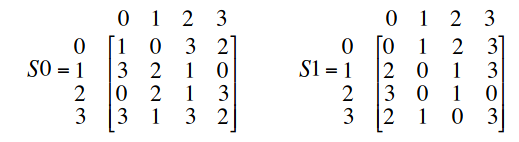
\includegraphics[width=0.8\textwidth]{imgs/s0_and_s1.png}
        \centering
        \label{fig:s0_and_s1}
    \end{figure} \\
    Sendo \texttt{wxyz} uma entrada, os valores de \texttt{w} e \texttt{z}
    correspondem à linha do \textit{S-box}, enquanto \texttt{x} e \texttt{y}
    correspondem à coluna. Por exemplo, sendo a entrada da \textit{S-box} a
    sequência \texttt{0001}, então \texttt{wz = 01} e \texttt{xy = 00}, assim,
    o resultado está na linha de número um e coluna número zero da matriz $S1$,
    resultando em 2, que em binário é \texttt{10}, portanto, \texttt{s = 1} e
    \texttt{t = 0}. Montando toda essa relação em uma tabela verdade: \\
    \begin{center}
        \begin{tabular}{c|c|c|c|c|c}
            w & x & y & z & s & t \\
            
            \hline
            0 & 0 & 0 & 0 & 0 & 0 \\
            0 & 0 & 0 & 1 & 1 & 0 \\
            0 & 0 & 1 & 0 & 0 & 0 \\
            0 & 0 & 1 & 1 & 0 & 0 \\
            0 & 1 & 0 & 0 & 1 & 0 \\
            0 & 1 & 0 & 1 & 0 & 1 \\
            ... & ... & ... & ... & ... & ... \\
            1 & 1 & 0 & 1 & 0 & 0 \\
            1 & 1 & 1 & 0 & 0 & 0 \\
            1 & 1 & 1 & 1 & 1 & 1 \\
        \end{tabular}
    \end{center}
    Com a tabela verdade acima, é possível montar um mapa de
    Karnaugh\cite{karnaugh1953} e dele derivar as equações para \texttt{s} e
    \texttt{t}, porém, o resultado estará na forma normal disjuntiva. Segue as
    equações para as variáveis \texttt{s} e \texttt{t}:
    \begin{gather*}
        s = \overline{xy}z + \overline{w}x\overline{z} + xyz + w\overline{xy}, \\
        t = \overline{w}y\overline{z} + \overline{w}xz + w\overline{yz} + wyz.
    \end{gather*}

    \item[3.18] Dado o texto cifrado $c =$ \texttt{10100010} e a chave $k =$
        \texttt{0111111101}, iremos decifrar a mensagem $c$ usando o
        \textit{simplifified DES}. Dada a estrutura do SDES, começando pela
        parte de geração de chaves:
    
    \begin{enumerate}
        \item \textbf{Permutação de 10 bits}: Ao aplicar a função de permutação
            de 10 bits na chave: \\
        $P10(k) = 1111110011$;
        \item \textbf{Deslocamento circular de 1 bit à esquerda}: Aplicando
            deslocamento circular de 1 bit nas partições \texttt{11111} e
            \texttt{10011}: \\
        $LS1(11111) = 11111$ e $LS1(10011) = 00111$;
        \item \textbf{Permutação de 8 bits}: A função de permutação de 8 bits
            nas duas partições anteriores e resultando na subchave $k_{1}$: \\
        $P8_{a}(11111, 00111) = 01011111$;
        \item \textbf{Deslocamento circular de 2 bits à esquerda}: As duas
            partições \texttt{11111} e \texttt{10011} têm os 2 bits deslocados
            à esquerda: \\
        $LS2(11111) = 11111$ e $LS2(10011) = 00111$;
        \item \textbf{Permutação de 8 bits}: Por fim, ambas as partições do
            item anterior são concatenadas e permutadas, resultado na subchave
            $k_{2}$: \\
        $P8_{b}(11111, 00111) = 11111100$.
    \end{enumerate}
    
    Seguindo com a estrutura do SDES:
    \begin{enumerate}
        \item \textbf{Permutação inicial}: O texto cifrado $c$ de 8 bits é
            entrada da função \texttt{IP} que realiza a permutação inicial: \\
        $IP(c) = 00110001$;
        \item \textbf{Expansão e permutação}: Os 4 bits menos significativos do
            resultado da permutação de $c$ do item anterior é entrada da função
            \texttt{E/P}, que realiza a expansão para 8 bits e permuta-os: \\
        $E/P(0001) = 10000010$;
        \item \textbf{XOR}: Realizando a operação de ou-exclusivo
            (\textit{XOR}) com o resultado do item anterior e a subchave
            $k_{2}$: \\
        $10000010 \oplus k_{2} = 01111110$;
        \item \textbf{\textit{S-boxes}}: Os bits mais e menos significativos do
            resultado da operação XOR anterior são entradas para as funções
            $S0$ e $S1$, respectivamente. Dos quatro bits, o quarto e o
            primeiro bits correspondem à linha da S-box, enquanto os dois bits
            do meio restantes correspondem à coluna: \\
        $S0(01, 11) = 00$ e $S1(10, 11) = 00$;
        \item \textbf{Permutação de 4 bits}: Os quatro bits resultantes do
            passo anterior são concatenados e permutados: \\
        $P4(00, 00) = 0000$;
        \item \textbf{XOR}: Por fim, há a operação de ou-exclusivo (XOR) entre
            os quatro bits do passo anterior e o os quatro bits mais
            significativos resultantes da permutação inicial do texto cifrado
            $c$: \\
        $0011 \oplus 0000 = 0011$.
    \end{enumerate}

    A função \texttt{Switch} recebe o resultado final da última operação XOR e
    os 4 bits menos significativos resultantes da permutação inicial do texto
    cifrado $c$. Nesta função os 4 bits menos significativos passam a ser os
    mais significativos e vice-versa: \\
    $SW(0011, 0001) = 00010011$
    
    Seguindo a estrutura final do SDES:
    \begin{enumerate}
        \item \textbf{Expansão e permutação}: Os 4 bits menos significativos do
            resultado da função \texttt{Switch} são entradas desta função: \\
        $E/P(0011) = 10010110$;
        \item \textbf{XOR}: Realizando a operação de ou-exclusivo (XOR) entre a
            subchave $k_{1}$ e o resultado do passo anterior: \\
        $10010110 \oplus k_{2} = 11001001$;
        \item \textbf{\textit{S-Boxes}}: Os bits mais e menos significativos do
            resultado da operação XOR anterior são entradas para as funções
            $S0$ e $S1$, respectivamente. Dos quatro bits, o quarto e o
            primeiro bits correspondem à linha da S-box, enquanto os dois bits
            do meio restantes correspondem à coluna: \\
        $S0(10, 10) = 01$ e $S1(11, 00) = 10$;
        \item \textbf{Permutação de 4 bits}: Os quatro bits resultantes do
            passo anterior são concatenados e permutados: \\
        $P4(0110) = 1010$
        \item \textbf{XOR}: Há a operação de ou-exclusivo (XOR) entre os quatro
            bits do passo anterior e o os quatro bits mais significativos
            resultantes da função \texttt{Switch}: \\
        $0001 \oplus 1010 = 1011$
        \item \textbf{$IP^{-1}$}: Por fim, é realizado a inversa da permutação
            inicial com a concatenação do resultado anterior e com os 4 bits
            menos significativos resultantes da função \texttt{Switch}: \\
        $IP^{-1}(1011,0011) = 11101010$.
    \end{enumerate}
    O texto decifrado é \texttt{11101010}, sendo que a cada quatro bits
    corresponde a uma codificação a uma letra do alfabeto, assim, \texttt{1110}
    corresponde à letra \texttt{O} e \texttt{1010} corresponde à letra
    \texttt{K}. Portanto o texto final decifrado é \texttt{OK}. 
\end{enumerate}

\bibliographystyle{acm}
\bibliography{01-des}

\end{document}
